\documentclass{article}
\usepackage{enumerate}
\usepackage{tikz}
\usetikzlibrary{graphs} 
\title{Hamiltonian Cycles in Square Lattice Subgraphs}
\begin{document}
\date{\vspace{-5ex}}
\maketitle

\section{Abstract}
This paper identifies a certain visual property of boundaries of right-angled walls, found in the video game Pacman, where corners are rounded and walls are straight and clamped towards the normal of the path which they face. The walls form a closed boundary. The 2-dimensional gridded nature of wall placement allows them to be represented using a square-lattice graph. With the aim of finding the direction towards which they are clamped, so as to recreate the visual properties of the walls in Pacman, we devise a polynomial-complexity algorithm for finding a hamiltonian cycle in square-lattice subgraphs, and establish the criteria for its devisability.

\section{Definitions}
\begin{enumerate}[I.]
\item We define a graph as a set $G=\lbrace V,E \rbrace$. $V$ is the set of vertices. $E$ is the set of edges. For an edge $e\in E, $ where $ V_{x},V_{y}\in V, e=\lbrace V_{x},V_{y} \rbrace $, means there is a connection between vertices $V_{x}$ and $V_{y}$. A graph can be represented by a drawing. For the example graph $G=\lbrace E,V \rbrace$, where $E=\lbrace a,b,c,d \rbrace $ and $ V=\{\{a,b\},\{b,c\},\{c,d\},\{d,a\},\{a,c\},\{d,b\}\}$ we can draw the following diagram.
\begin{figure}[h]
\centering
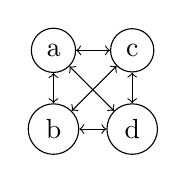
\begin{tikzpicture} \graph[nodes={draw,circle}] {{a,b}<->{c,d},{a,c}<->{d,b},{a,c}<->{b,d}}; \end{tikzpicture}
\caption{A graph of four vertices that are all bidirectionally connected to each other.}
\end{figure}
\item We define a lattice graph as a graph L in which ...
\end{enumerate}
\end{document}